\graphicspath{{./chapitres/chapitre5/figures/}}
\setcounter{mtc}{4}
\chapter{Sprint\textcolor{white}{J}Deux : Développement\textcolor{white}{J}de\textcolor{white}{J}la partie backend }
\fancyhead[R]{\ungaramond\small\textbf{Chapitre\textcolor{white}{J}4: Développement de la partie backend }}
\minitoc
\newpage
\section*{Introduction}
Nous continuons la phase de réalisation de ce projet par le deuxième sprint où on va se focaliser sur le développement de la partie backend ainsi que la communication avec le moteur graphique en les détaillant par la backlog produit et le diagramme de cas d’utilisation raffiné pour chaque cas d’utilisation pour finir avec quelques captures d’écran de chaque cas d’utilisation.

\section{Sprint  Backlog}
\subsection{Histoires\textcolor{white}{J}\`a\textcolor{white}{J}r\'ealiser}

La\textcolor{white}{J}liste\textcolor{white}{J}des\textcolor{white}{J}tâches\textcolor{white}{J}à\textcolor{white}{J}réaliser\textcolor{white}{J}dans\textcolor{white}{J}le\textcolor{white}{J}sprint\textcolor{white}{J}deux est\textcolor{white}{J}décrite\textcolor{white}{J}dans\textcolor{white}{J}le\textcolor{white}{J}tableau \ref{tab:sprint_4_backlog} \textcolor{white}{J}.

\begin{longtable}[!ht]{|m{1cm}|m{3cm}|m{1cm}|m{7cm}|m{1.3cm}|}
\hline
{\textbf{Id story}} & {\textbf{User story}} & {\textbf{id tâche}} & {\textbf{tâche}} & {\textbf{estima-tion(H)}}\\
\hline
1.1 & En tant qu’utilisateur je souhaite sauvegarder la session  & 1.1.1 & Initiation et configuration des projets de la partie backend & 6\\
\cline{3-5}
&   & 1.1.2 & Mise en place de l’architecture cible & 2\\
\cline{3-5}
&	& 1.1.3 & Développement de la partie Backend & 8\\
\cline{3-5}
&	& 1.1.4 & Communication avec le moteur graphique & 4\\
\cline{3-5}
&	& 1.1.5 & Intégration du protocole d’autorisation OAuth2 & 10\\
\cline{3-5}
&	& 1.1.6 & Validation du token et renvoie des images au client & 10\\
\cline{3-5}
&	& 1.1.7 & Configuration de la base de données No SQL Cosmos DB & 1\\
\cline{3-5}
&	& 1.1.8 & Connecter la partie backend a la base de données & 4\\
\cline{3-5}
&	& 1.1.9 & Créer l’API de sauvegarde des simulations & 1\\
\hline
\caption{Liste des tâches du deuxième Sprint}
\label{tab:sprint_4_backlog}
\end{longtable}

\section{Conception}
\subsection{Diagrammes\textcolor{white}{J}d’activié}
Le\textcolor{white}{J}schema\textcolor{white}{J}  \ref{fig:digAct4} suivant\textcolor{white}{J}présente\textcolor{white}{J}le\textcolor{white}{J}diagramme\textcolor{white}{J}d’activité
\begin{figure}[!ht]\centering
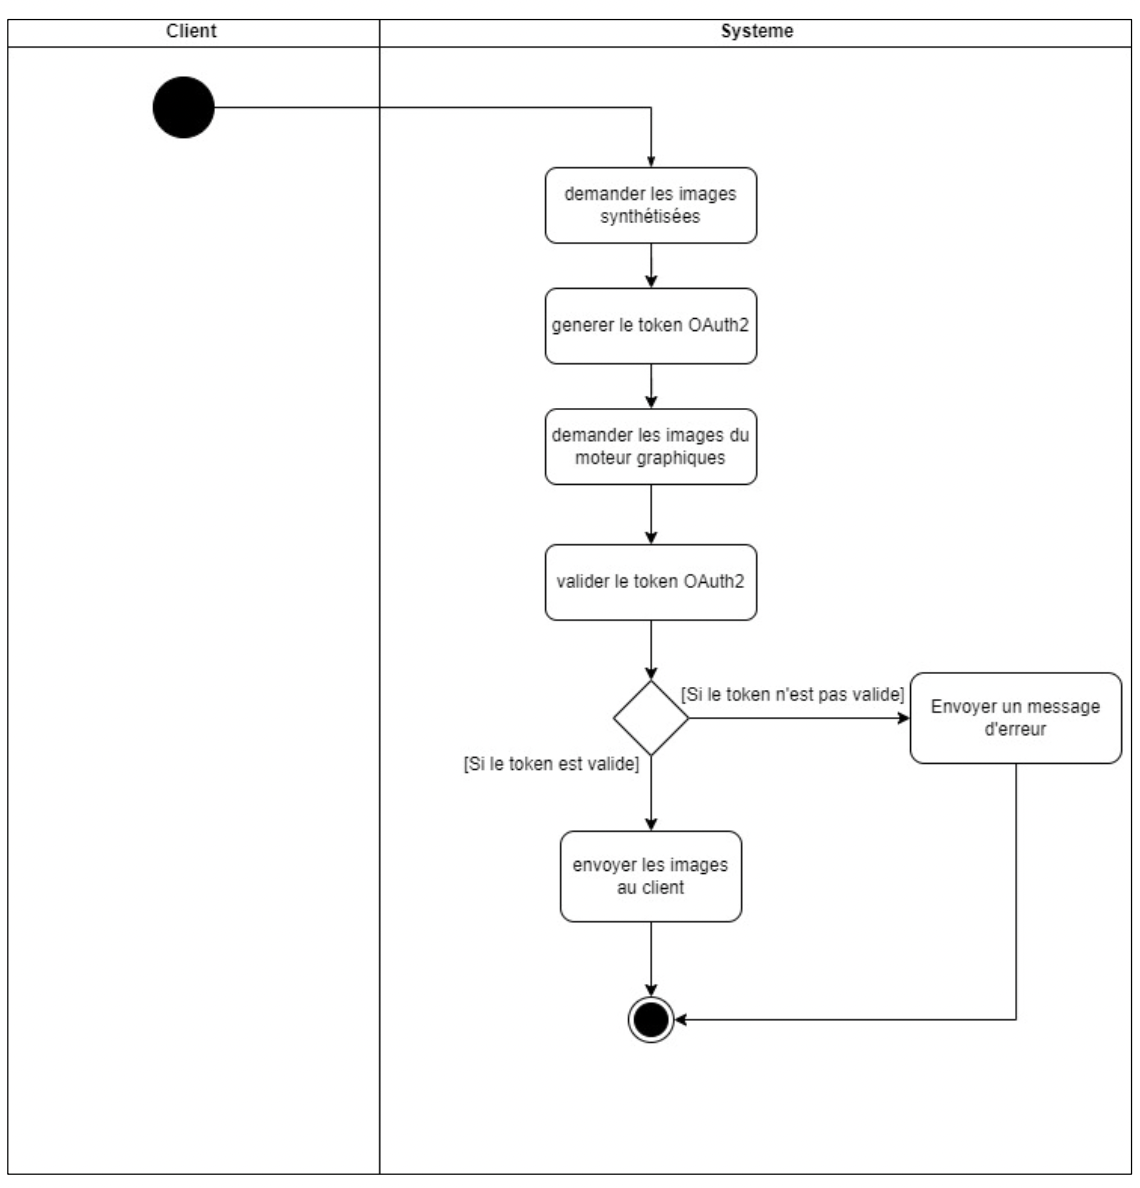
\includegraphics[width=1\textwidth,angle=00]{chapitres/chapitre4/figures/Act-Chap4.png}
\caption{Diagramme\textcolor{white}{J}d’activité}
\label{fig:digAct4}
\end{figure}

en demandant les images synthétisées,le systeme va generer une  clé d'authentification puis demander les images du moteur graphiques et les envoyer a la partie backend.Ensuite,le serveur backend procede a la validation de la cle d'authentification.Si la clé n'est pas valide,un message d'erreur est envoyé au client.Sinon les images synthétisées sont envoyées au client.

\newpage
\subsection{Diagramme\textcolor{white}{J}de\textcolor{white}{J}séquence\textcolor{white}{J}objet}
\begin{figure}[!ht]\centering
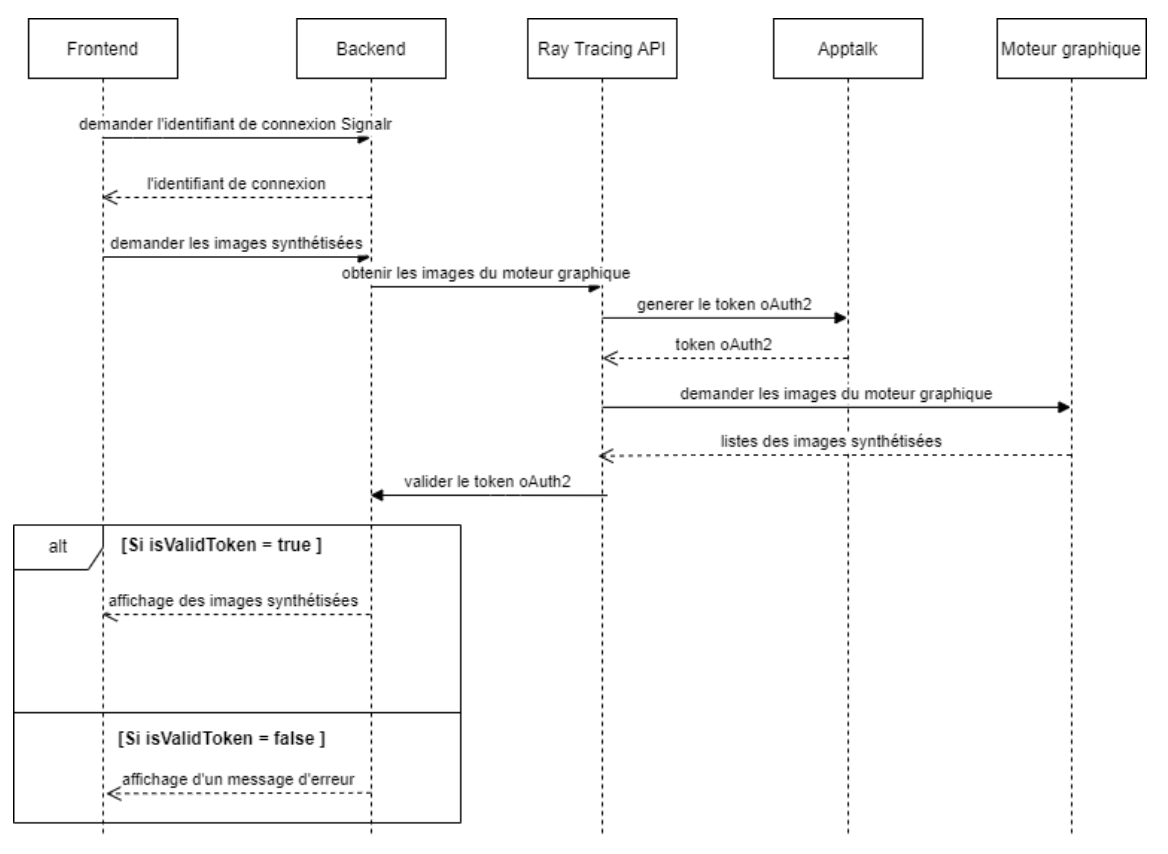
\includegraphics[width=0.8\textwidth,angle=00]{chapitres/chapitre4/figures/Seq-Chap4.png}
\caption{Diagramme\textcolor{white}{J}de\textcolor{white}{J}séquence\textcolor{white}{J}objet
}
\label{fig:schemaSourcin}
\end{figure}


\subsection{Diagramme\textcolor{white}{J}de\textcolor{white}{J}séquence\textcolor{white}{J}de\textcolor{white}{J}la demande du jeton d’accès}
\begin{figure}[!ht]\centering
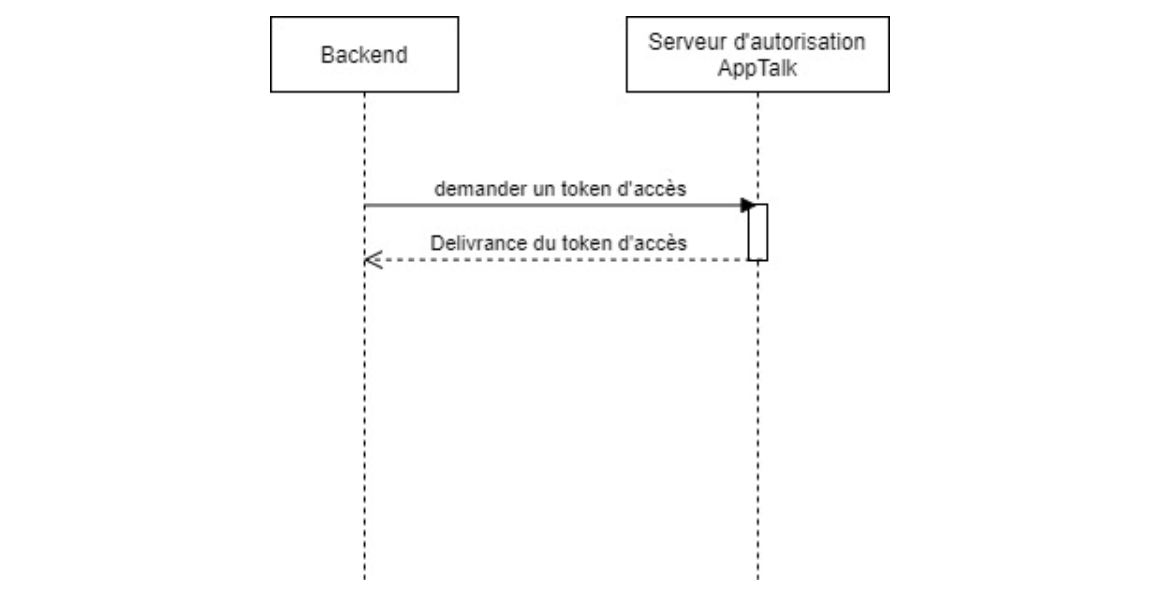
\includegraphics[width=0.9\textwidth,angle=00]{chapitres/chapitre4/figures/SeqDemande-Chap4.png}
\caption{Diagramme de séquence de la demande du jeton d’accès}
\label{fig:schemaSourcin}
\end{figure}

\newpage
\subsection{Diagramme\textcolor{white}{J}de\textcolor{white}{J}classe\textcolor{white}{J}de\textcolor{white}{J}conception}
\begin{figure}[!ht]\centering
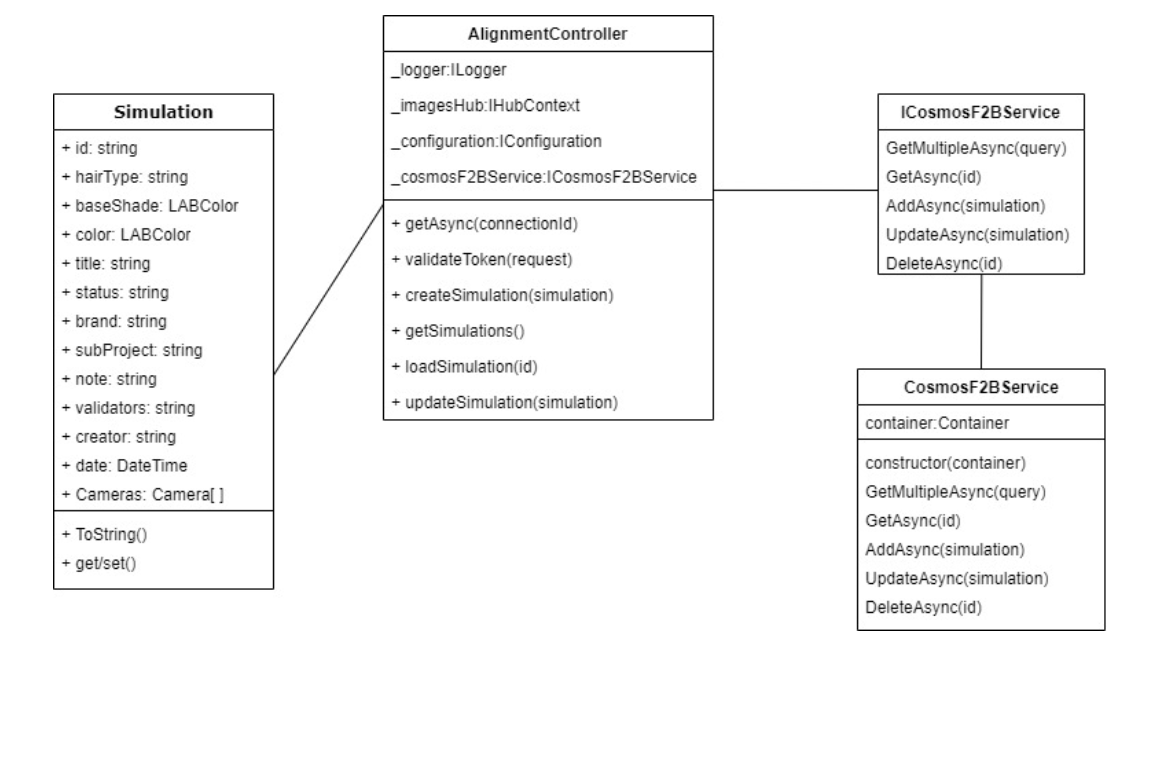
\includegraphics[width=0.9\textwidth,angle=00]{chapitres/chapitre4/figures/Class-Chap4.png}
\caption{Diagramme\textcolor{white}{J}de\textcolor{white}{J}classe\textcolor{white}{J}de\textcolor{white}{J}conception}
\label{fig:schemaSourcin}
\end{figure}

\section{Réalisation}

\subsection{Technologies}
\subsubsection*{Swagger[11]}
À l’heure actuelle, Swagger est la meilleure solution pour documenter une API REST, car le système est capable de représenter presque tous les services Web et informations ayant trait à l’interface. La documentation évolue en même temps que le système et enregistre automatiquement les modifications. Swagger se montre particulièrement efficace pour parvenir à ce résultat parce qu’il consigne la documentation d’une API REST directement dans son code. Grace au fichier Swagger.json qui contient toutes les informations sur nos APIs, on peut générer le client HTTP pour accéder aux APIs dans le Frontend en utilisant le package Autorest.


\newpage
\subsubsection*{SignalR[12]}
SignalR est une bibliothèque client/serveur pour Microsoft ASP.NET qui permet au code serveur d'envoyer des notifications asynchrones aux applications Web côté client. La bibliothèque comprend des composants JavaScript côté serveur et côté client. Il fournit également une API simple et de haut niveau pour effectuer des RPC de serveur à client (appeler des fonctions JavaScript dans le navigateur d'un client à partir du code .NET côté serveur) dans une application ASP.NET, ainsi que l'ajout de fonctions utiles pour la gestion des connexions tels que les événements de connexion/déconnexion et l’autorisation.



\subsubsection*{Cosmos DB[13]}
Azure Cosmos DB est une base de données NoSQL sans serveur, entièrement gérée, destinée aux applications hautes performances avec une vitesse garantie à n’importe quelle échelle avec un débit instantané et illimité, des lectures rapides et des écritures multirégion partout dans le monde.
Avec des kits de développement logiciel (SDK) pour les langages les plus courants, ainsi qu'une API Core (SQL) native, des API pour MongoDB, Cassandra et Gremlin



\newpage
\subsection{Mise en place de l’architecture cible}
Après l’évolution de l’application OptixHair en un moteur graphique capable d’envoyer les images dans un bus de communication instantanée appelée websocket, on a développé la partie backend qui doit communiquer avec ce dernier.
La partie backend est divisée en deux parties : 
Une partie responsable a la communication avec le client intitulé Backend API et une partie qui communiquera avec le moteur graphique qui s’appelle SimulatorInterface API.
La figure \ref{fig:cible} suivante représente l’architecture cible de ce sprint.

\begin{figure}[!ht]\centering
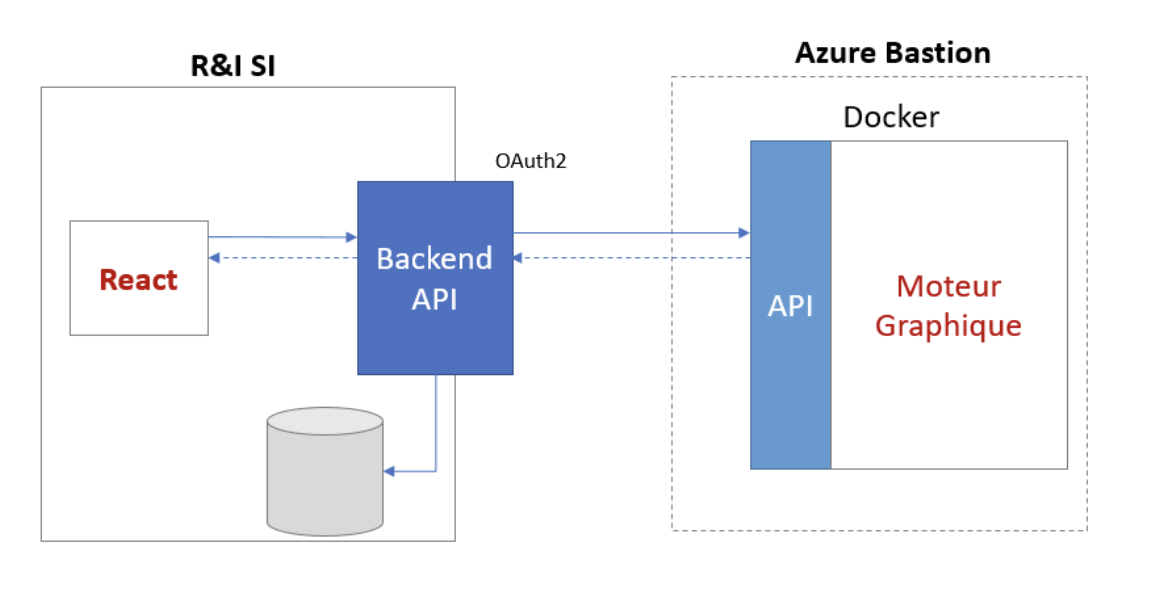
\includegraphics[width=0.9\textwidth]{chapitres/chapitre4/figures/ArchCible.png}
\caption{L’architecture cible}
\label{fig:cible}
\end{figure}

\subsection{Implémentation}
\subsubsection{Développement de la partie Backend}

Tout d’abord, on a développé une API fonctionnelle responsable de la communication entre le serveur Backend et le serveur de communication avec le moteur graphique. Cette API est exposée avec la méthode GET du protocole http sous le chemin « /Alignement/Get/ » et prend en paramètre l’identifiant de connexion du client qui demande les images synthétisées. 
La figure suivante représente l’API de récupération des images.

\begin{figure}[!ht]\centering
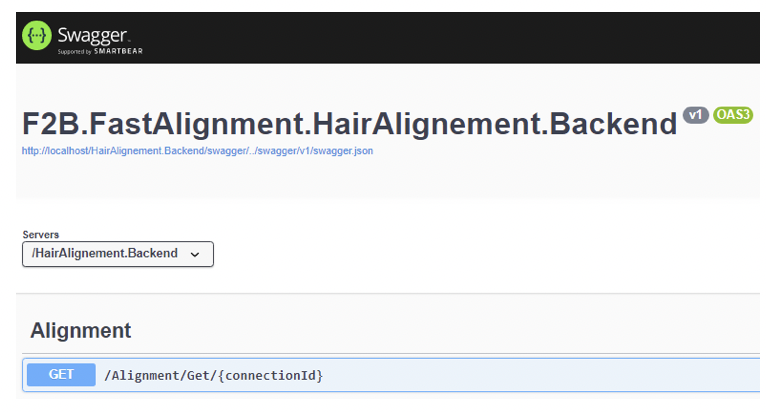
\includegraphics[width=0.8\textwidth]{chapitres/chapitre4/figures/AlignementGet.png}
\caption{Récupération des images}
\label{fig:git}
\end{figure}

Dans cette API, on a exécuté une requête au serveur « SimulatorInterface API » pour qu’il récupère les images synthétisées du moteur graphique et les renvoyés au serveur « Backend API » puis ce dernier va faire la redirection de ses images au client.

\subsubsection{ Intégration du protocole d’autorisation OAuth2}
Pour assurer l’authentification de cette communication, on a utilisé OAuth2 qui est un protocole d’autorisation largement utilisé par L’Oréal.
La demande d'accès à une ressource protégée avec ce protocole se traduit par l'émission d'un jeton au client. Le jeton représente simplement une chaîne unique utilisée pour identifier le client et diverses informations utiles lors du processus d'autorisation. Ce dernier a une durée de validité limitée.
Pour en obtenir un, le serveur « SimulatorInterface API » doit faire une requête au serveur d’autorisation AppTalk en précisant ces paramètres.

\begin{figure}[!ht]\centering
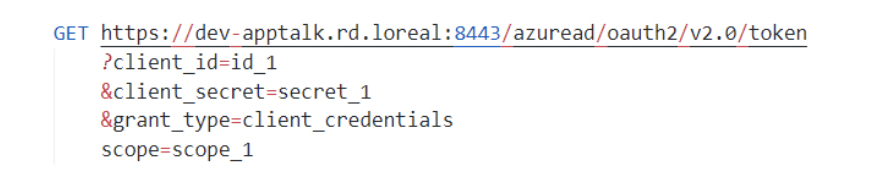
\includegraphics[width=0.8\textwidth]{chapitres/chapitre4/figures/Apptalk.png}
\caption{Récupération des images}
\label{fig:git}
\end{figure}

Si tout se passe bien, l’AppTalk renverrait une réponse contenant notre token d’accès.

\begin{figure}[!ht]\centering
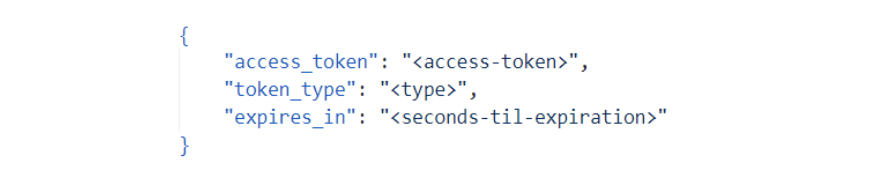
\includegraphics[width=0.8\textwidth]{chapitres/chapitre4/figures/Apptalk-token.png}
\caption{Récupération des images}
\label{fig:git}
\end{figure}

\subsubsection{ Communication avec le moteur graphique}
Après avoir récupérer le jeton d’accès, le serveur « SimulatorInterface API » va ouvrir une session de communication instantanée avec le moteur graphique pour récupérer les images synthétisées puis les renvoyées au serveur « Backend API » tout en spécifiant le jeton d’accès à l’entête. 

La figure \ref{fig:comMoteur} suivante représente l’API de communication avec le moteur graphique.

\begin{figure}[!ht]\centering
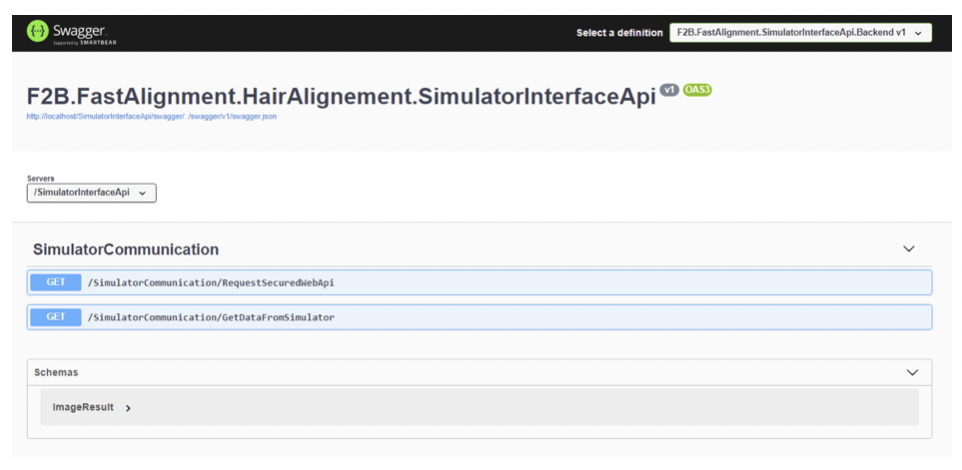
\includegraphics[width=0.7\textwidth]{chapitres/chapitre4/figures/SimuGet.png}
\caption{Communication avec le moteur graphique}
\label{fig:comMoteur}
\end{figure}

\subsubsection{ Validation du token et renvoie des images au client}
Maintenant, le serveur « Backend API » doit tout d’abord vérifier la validité du token via l’API « validateToken », si le token est valide les images seront publiées au client le bus de communication SignalR. Dans le cas contraire une exception sera levée, l’envoie des images sera abandonné et le message d’erreur sera envoyé au client.
La figure \ref{fig:vldToken} ci-dessous représente l’API de validation du token « validateToken ».

\begin{figure}[!ht]\centering
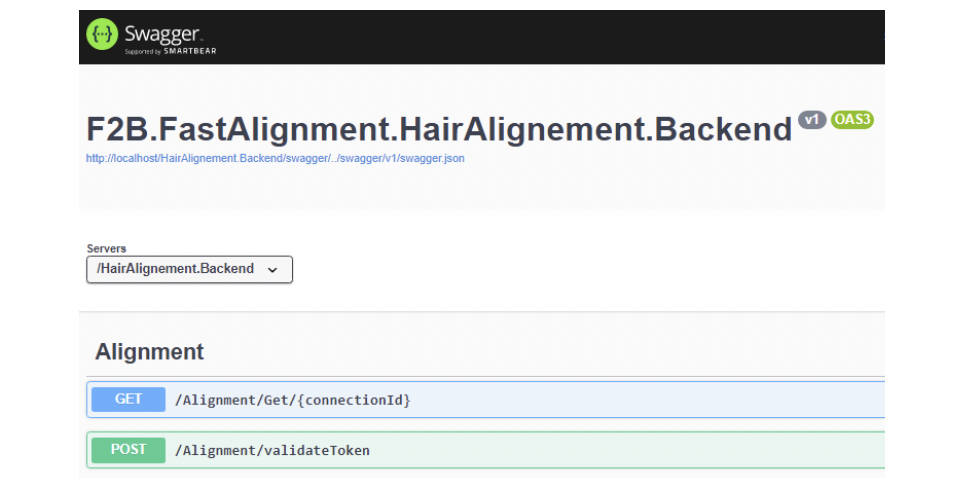
\includegraphics[width=0.7\textwidth]{chapitres/chapitre4/figures/AlignementPost.png}
\caption{Api de validation du token}
\label{fig:vldToken}
\end{figure}

\newpage
\subsubsection{ Configuration de la base de données Cosmos DB}
Pour le stockage des simulations, on a opté pour la base de données Cosmos DB qui est une base de données NoSQL distribué mondialement. Azure Cosmos DB est disponible dans toutes les régions Azure à travers le monde.
Azure Cosmos DB organise les données dans une structure hiérarchique de bases de données, de conteneurs et d'éléments. Nous pouvons ajouter une base de données, des conteneurs et des éléments à partir du panneau Data Explorer de Cosmos DB.
La figure \ref{fig:comCosmos} suivante présente le conteneur créé intitulé F2BContainer

\begin{figure}[!ht]\centering
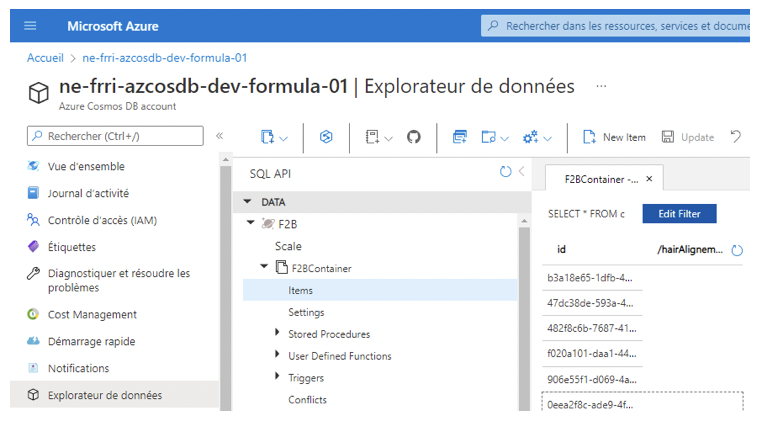
\includegraphics[width=0.8\textwidth]{chapitres/chapitre4/figures/Azure.png}
\caption{Configuration de la base de données Cosmos DB}
\label{fig:comCosmos}
\end{figure}

Maintenant que nous avons créé le conteneur, nous devons ajouter les packages NuGet nécessaires pour se connecter à Azure Cosmos DB.

\begin{figure}[!ht]\centering
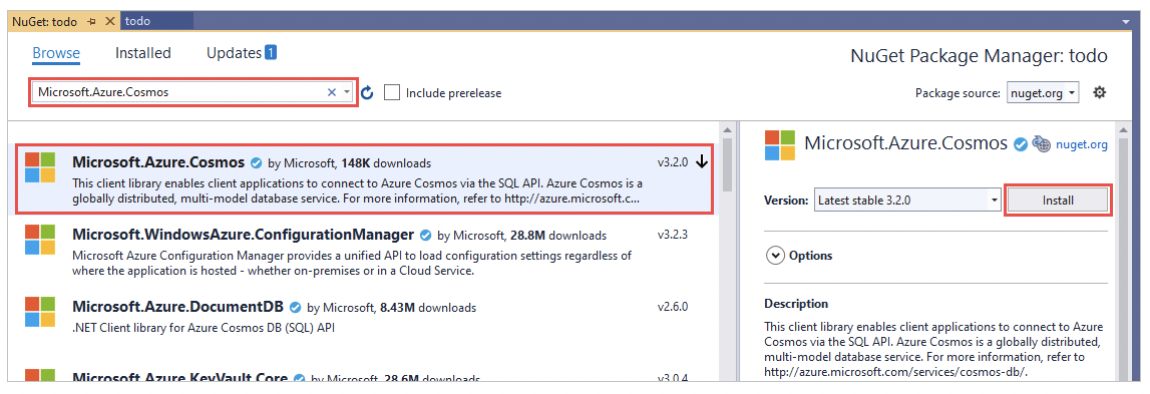
\includegraphics[width=0.8\textwidth]{chapitres/chapitre4/figures/CosmosDB.png}
\caption{Configuration de la base de données Cosmos DB}
\label{fig:git}
\end{figure}

\newpage
Ensuite, nous avons ajouté une classe qui contient la logique pour se connecter et utiliser Azure Cosmos DB. Dans ce didacticiel, nous avons encapsulé cette logique dans une classe appelée « CosmosF2BService » et une interface appelée « ICosmosF2BService ». Ce service effectue des opérations CRUD. Il effectue également des opérations de lecture de flux telles que la liste des éléments incomplets, la création, la modification et la suppression d'éléments.

Nous avons aussi ajouté la méthode « InitializeCosmosClientInstanceAsync » pour créer un client cosmos comme indiqué dans la figure ci-dessous. Cette fonction a besoin de ces paramètres pour pouvoir créer l’instance de connexion :
\begin{figure}[!ht]\centering
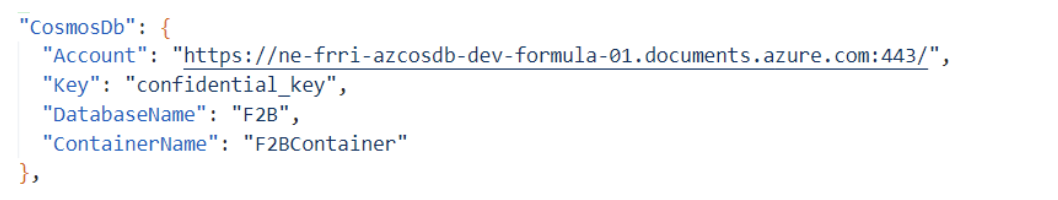
\includegraphics[width=0.8\textwidth]{chapitres/chapitre4/figures/CosmosDb-azure.png}
\caption{InitializeCosmosClientInstanceAsync}
\label{fig:git}
\end{figure}

\subsubsection{Créer l’API de sauvegarde des simulations}
Pour utiliser les opérations CRUD qu’on a implémenté dans le service « CosmosF2BService », on a déclaré une variable de l’interface ce service en « readonly » pour faire l’injection de dépendance. Par la suite, on a créé quatre APIs fonctionnelles où on a fait l’appel des fonctions du service « CosmosF2BService »
La figure \ref{fig:crud} ci-dessous présente les APIs des opérations CRUD

\begin{figure}[!ht]\centering
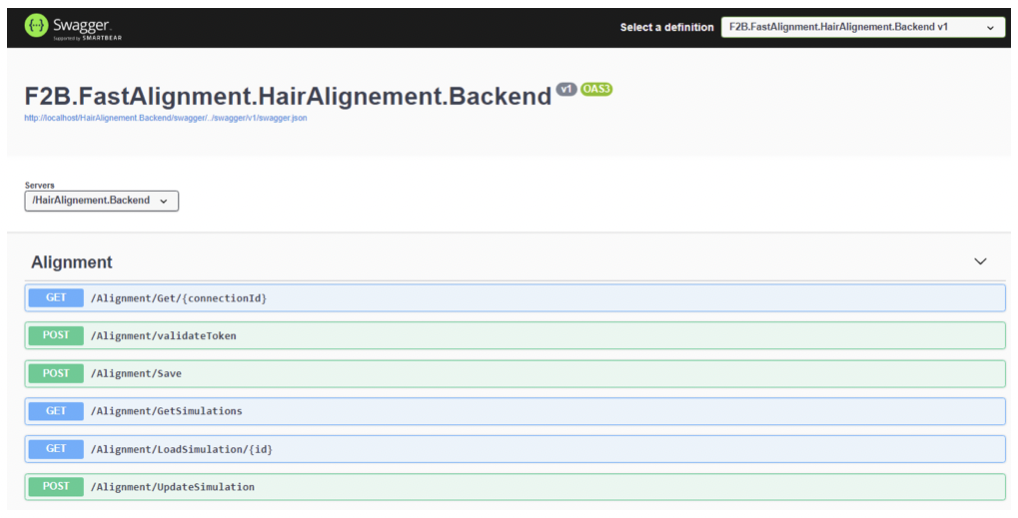
\includegraphics[width=0.8\textwidth]{chapitres/chapitre4/figures/crud.png}
\caption{Les opérations CRUD}
\label{fig:crud}
\end{figure}


\section*{Conclusion}
Au cours de ce chapitre, nous avons réussi à développer la partie backend qui comporte la gestion des simulations et la mise en place du protocole d’authentification OAuth2. Dans le chapitre suivant, tout l’effort sera consacré pour développer la partie frontend puis l’intégration du projet dans la Formulation Center et enfin le déploiement de notre solution.


